\let\negmedspace\undefined
\let\negthickspace\undefined
\documentclass[journal]{IEEEtran}
\usepackage[a5paper, margin=10mm, onecolumn]{geometry}
%\usepackage{lmodern} % Ensure lmodern is loaded for pdflatex
\usepackage{tfrupee} % Include tfrupee package

\setlength{\headheight}{1cm} % Set the height of the header box
\setlength{\headsep}{0mm}     % Set the distance between the header box and the top of the text

\usepackage{gvv-book}
\usepackage{gvv}
\usepackage{cite}
\usepackage{amsmath,amssymb,amsfonts,amsthm}
\usepackage{algorithmic}
\usepackage{graphicx}
\usepackage{textcomp}
\usepackage{xcolor}
\usepackage{txfonts}
\usepackage{listings}
\usepackage{enumitem}
\usepackage{mathtools}
\usepackage{gensymb}
\usepackage{comment}
\usepackage[breaklinks=true]{hyperref}
\usepackage{tkz-euclide} 
\usepackage{listings}
                                         
\def\inputGnumericTable{}                                 
\usepackage[latin1]{inputenc}                                
\usepackage{color}                                            
\usepackage{array}                                            
\usepackage{longtable}                                       
\usepackage{calc}                                             
\usepackage{multirow}                                         
\usepackage{hhline}                                           
\usepackage{ifthen}                                           
\usepackage{lscape}
\begin{document}


\bibliographystyle{IEEEtran}

\title{9.4.34}
\author{EE25BTECH11021 - Dhanush sagar}
% \maketitle
% \newpage
% \bigskip
\maketitle \vspace{-1cm}
\renewcommand{\thefigure}{\theenumi}
\renewcommand{\thetable}{\theenumi}
\setlength{\intextsep}{10pt} % Space between text and floats

\
\numberwithin{figure}{enumi}
\renewcommand{\thetable}{\theenumi}

\textbf{Question:}  \\
Rohan's mother is 26 years older than him. The product of their ages (in years) 3 years from now will be 360. We would like to find Rohan's present age.

\textbf{Solution:}  \\
Let the present ages be represented as the vector:
\begin{align}
\vec{x} = \myvec{x \\ y}
\end{align}
where $x$ and $y$ denote Rohan's and his mother's present ages respectively.\\

given,\\
eq 1 :Since the mother is 26 years older than Rohan,
\begin{align}
y = x + 26
\end{align}
eq 2 :The product of their ages three years from now is given as
\begin{align}
(x+3)(y+3) = 360
\end{align}

Expanding the above equation:
\begin{align}
xy + 3x + 3y - 351 = 0
\end{align}

This can be written in quadratic (matrix) form as
\begin{align}
\vec{x}^\top \vec{V} \vec{x} + 2\vec{u}^\top \vec{x} + f = 0
\end{align}
where
\begin{align}
\vec{V} = \myvec{0 & \tfrac{1}{2} \\[4pt] \tfrac{1}{2} & 0}, \quad
\vec{u} = \myvec{\tfrac{3}{2} \\[4pt] \tfrac{3}{2}}, \quad
f = -351
\end{align}

The line $y = x + 26$ can be expressed parametrically as
\begin{align}
\vec{x} = \vec{h} + \kappa \vec{m}, \quad \kappa \in \mathbb{R}
\end{align}
where
\begin{align}
\vec{h} = \myvec{0 \\ 26}, \quad \vec{m} = \myvec{1 \\ 1}
\end{align}

Substituting $\vec{x} = \vec{h} + \kappa \vec{m}$ in the conic equation:
\begin{align}
(\vec{h} + \kappa\vec{m})^\top \vec{V}(\vec{h} + \kappa\vec{m})
+ 2\vec{u}^\top (\vec{h} + \kappa\vec{m}) + f = 0
\end{align}

Grouping powers of $\kappa$, we get:
\begin{align}
\kappa^2 (\vec{m}^\top \vec{V}\vec{m})
+ 2\kappa\, \vec{m}^\top (\vec{V}\vec{h} + \vec{u})
+ g(\vec{h}) = 0
\end{align}
where
\begin{align}
g(\vec{h}) = \vec{h}^\top \vec{V}\vec{h} + 2\vec{u}^\top \vec{h} + f
\end{align}

Now compute each term:

\begin{align}
\vec{m}^\top \vec{V}\vec{m} &= 
\myvec{1 & 1}
\myvec{0 & \tfrac{1}{2} \\[4pt] \tfrac{1}{2} & 0}
\myvec{1 \\[4pt] 1}
= 1
\\[6pt]
\vec{V}\vec{h} + \vec{u} &=
\myvec{0 & \tfrac{1}{2} \\[4pt] \tfrac{1}{2} & 0}\myvec{0 \\[4pt] 26}
+ \myvec{\tfrac{3}{2} \\[4pt] \tfrac{3}{2}}
= \myvec{14.5 \\[4pt] 1.5}
\\[6pt]
\vec{m}^\top (\vec{V}\vec{h} + \vec{u}) &= \myvec{1 & 1}\myvec{14.5 \\[4pt] 1.5} = 16
\\[6pt]
g(\vec{h}) &= \vec{h}^\top \vec{V}\vec{h} + 2\vec{u}^\top \vec{h} + f
= 0 + 2(\tfrac{3}{2}\times 26) - 351 = -273
\end{align}

Substituting these results gives:
\begin{align}
\kappa^2 + 32\kappa - 273 = 0
\end{align}

The general quadratic solution is
\begin{align}
\kappa =
\dfrac{
-\,\vec{m}^\top (\vec{V}\vec{h} + \vec{u})
\pm
\sqrt{
\left[\vec{m}^\top (\vec{V}\vec{h} + \vec{u})\right]^2
- g(\vec{h})\,(\vec{m}^\top \vec{V}\vec{m})
}
}{
\vec{m}^\top \vec{V}\vec{m}
}
\end{align}

Substituting numerical values:
\begin{align}
\kappa =
\dfrac{-16 \pm \sqrt{16^2 - (-273)}}{1}
= -16 \pm \sqrt{529}
= -16 \pm 23
\end{align}

Thus,
\begin{align}
\kappa_1 = -39, \quad \kappa_2 = 7
\end{align}

The intersection points are
\begin{align}
\vec{x}_i = \vec{h} + \kappa_i \vec{m}, \quad i = 1,2
\end{align}

Hence,
\begin{align}
\vec{x}_1 = \myvec{0 \\ 26} - 39\myvec{1 \\ 1} = \myvec{-39 \\ -13}, \quad
\vec{x}_2 = \myvec{0 \\ 26} + 7\myvec{1 \\ 1} = \myvec{7 \\ 33}
\end{align}

The physically meaningful (non-negative) intersection corresponds to
\begin{align}
\boxed{x = 7, \quad y = 33}
\end{align}

Therefore, Rohan's present age is{7\text{ years}}and his mother's present age is{33\text{years}}.

\begin{figure}[H]
    \centering
    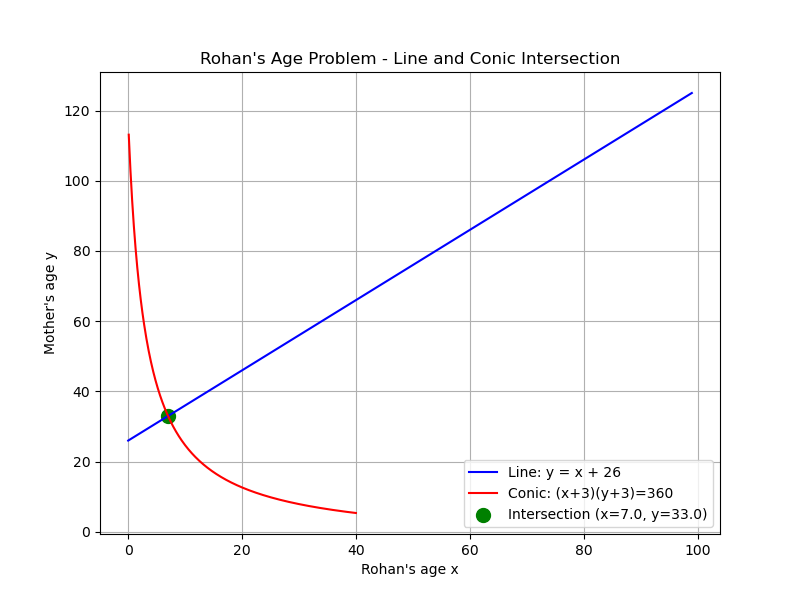
\includegraphics[width=0.8\columnwidth]{Figs/Fig1.png}
    \caption{}
    \label{fig:placeholder}
\end{figure}
\end{document}















